\documentclass[10pt]{article}
\usepackage[a4paper,margin=1.55cm]{geometry}
\usepackage{graphicx}
\usepackage{amsmath}
\usepackage{natbib}
\usepackage{microtype}
\usepackage{caption}
\captionsetup{font=small,skip=2pt}
\setlength{\parskip}{3pt}
\setlength{\parindent}{0pt}
\title{Nonlinear Dynamics of the Logistic Map and an Educational Interval-Mapping Text Demonstration}
\author{Course Project}
\date{}
\begin{document}
% Title and abstract occupy a separate page, as required.
\maketitle
\begin{abstract}
We numerically study the logistic map $x_{n+1}=rx_n(1-x_n)$ through a time series, bifurcation diagram, Lyapunov-exponent sweep, sensitivity experiment, trajectory-separation plot, and invariant-density estimate. At $r=4$, the computed Lyapunov exponent is 0.693020, close to $\ln 2=0.693147$, and the mean of 500,000 retained samples is 0.4992599, close to 0.5. We also test a small interval-mapping text demonstration: four messages are recovered exactly. This text experiment is explicitly educational only. It is neither a faithful reproduction of Baptista's 1998 cryptosystem nor evidence of security. Literature is reviewed separately from the performed simulations.
\end{abstract}
\vfill
\noindent\textbf{Keywords:} logistic map; bifurcation; Lyapunov exponent; invariant density; chaotic cryptography
\clearpage
% Main content: deliberately bounded to five pages (pp. 1--5).
\setcounter{page}{1}
\section{Introduction and model}
The logistic map is a compact model in which the control parameter $r$ changes the long-term behaviour from stable fixed points to periodic and chaotic regimes. We study
\begin{equation}
x_{n+1}=r x_n(1-x_n), \qquad 0\leq x_n\leq1 .
\end{equation}
For the single-orbit experiments, $r=4.0$ and $x_0=0.213$. The original chaos-based cipher of \citet{Baptista1998} encodes a symbol through an iteration count to a partition of the chaotic attractor. That idea motivates our final classroom demonstration, but not a security claim.
\section{Methods}
For each $r$ in a sweep, the largest Lyapunov exponent is estimated after a transient by averaging $\log |r(1-2x_n)|$. The bifurcation scan uses 3,000 values from 2.8 to 4.0, discards 1,000 iterates, and records 200 more at each value. The Lyapunov scan uses 3,000 values from 2.5 to 4.0, with 1,000 transient and 3,000 accumulation iterates. Sensitivity is tested from $0.213$ and $0.213+10^{-10}$ for 70 iterations.

For the invariant-density experiment, 1,000 transient iterates are removed and 500,000 states at $r=4$ are retained. The reference density is $\rho(x)=[\pi\sqrt{x(1-x)}]^{-1}$. All figures were generated by the submitted Colab-exported Python script and supplied results archive.
\begin{figure}[h]
\centering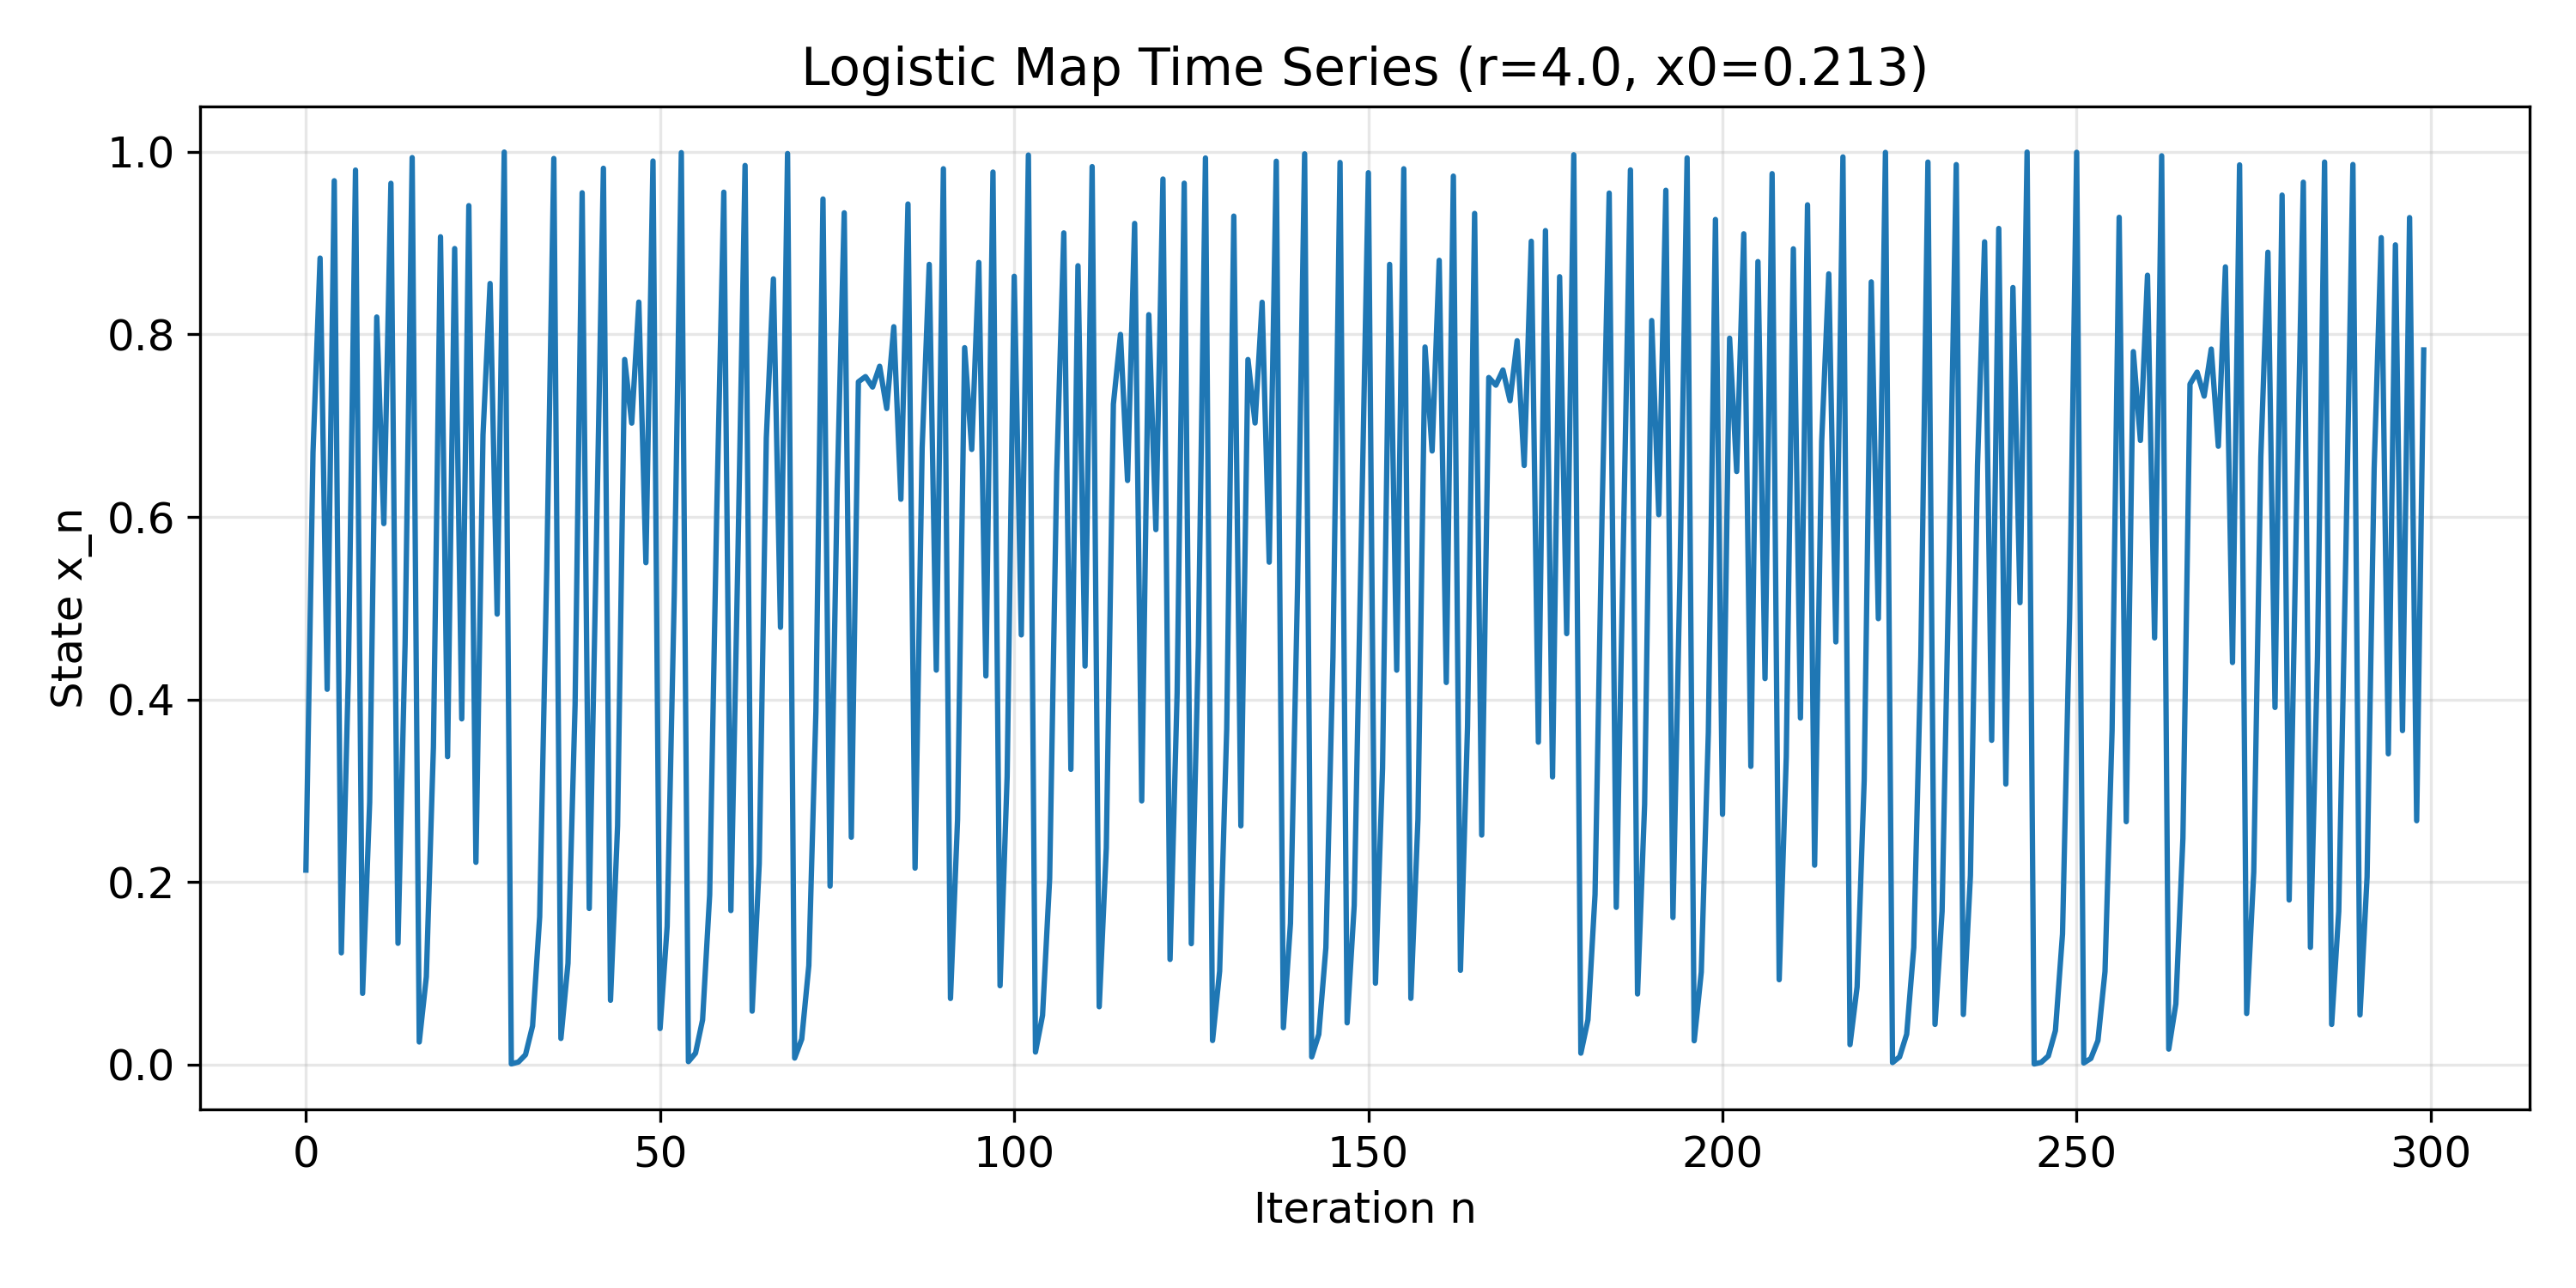
\includegraphics[width=.76\linewidth]{../results/logistic_map_timeseries.png}
\caption{Logistic-map time series for $r=4$ and $x_0=0.213$.}
\end{figure}
\section{Parameter dependence and instability}
The bifurcation diagram shows the changing long-term orbit structure as $r$ increases. The Lyapunov curve summarizes local exponential expansion or contraction. At $r=4$, the numerical estimate is 0.693020 versus the exact value $\ln2=0.693147$; their difference is consistent with finite sampling and floating-point computation. The two nearby trajectories visibly separate, while the logarithmic separation plot makes the early growth easier to inspect.
\begin{figure}[h]
\centering
\begin{minipage}{.49\linewidth}\centering
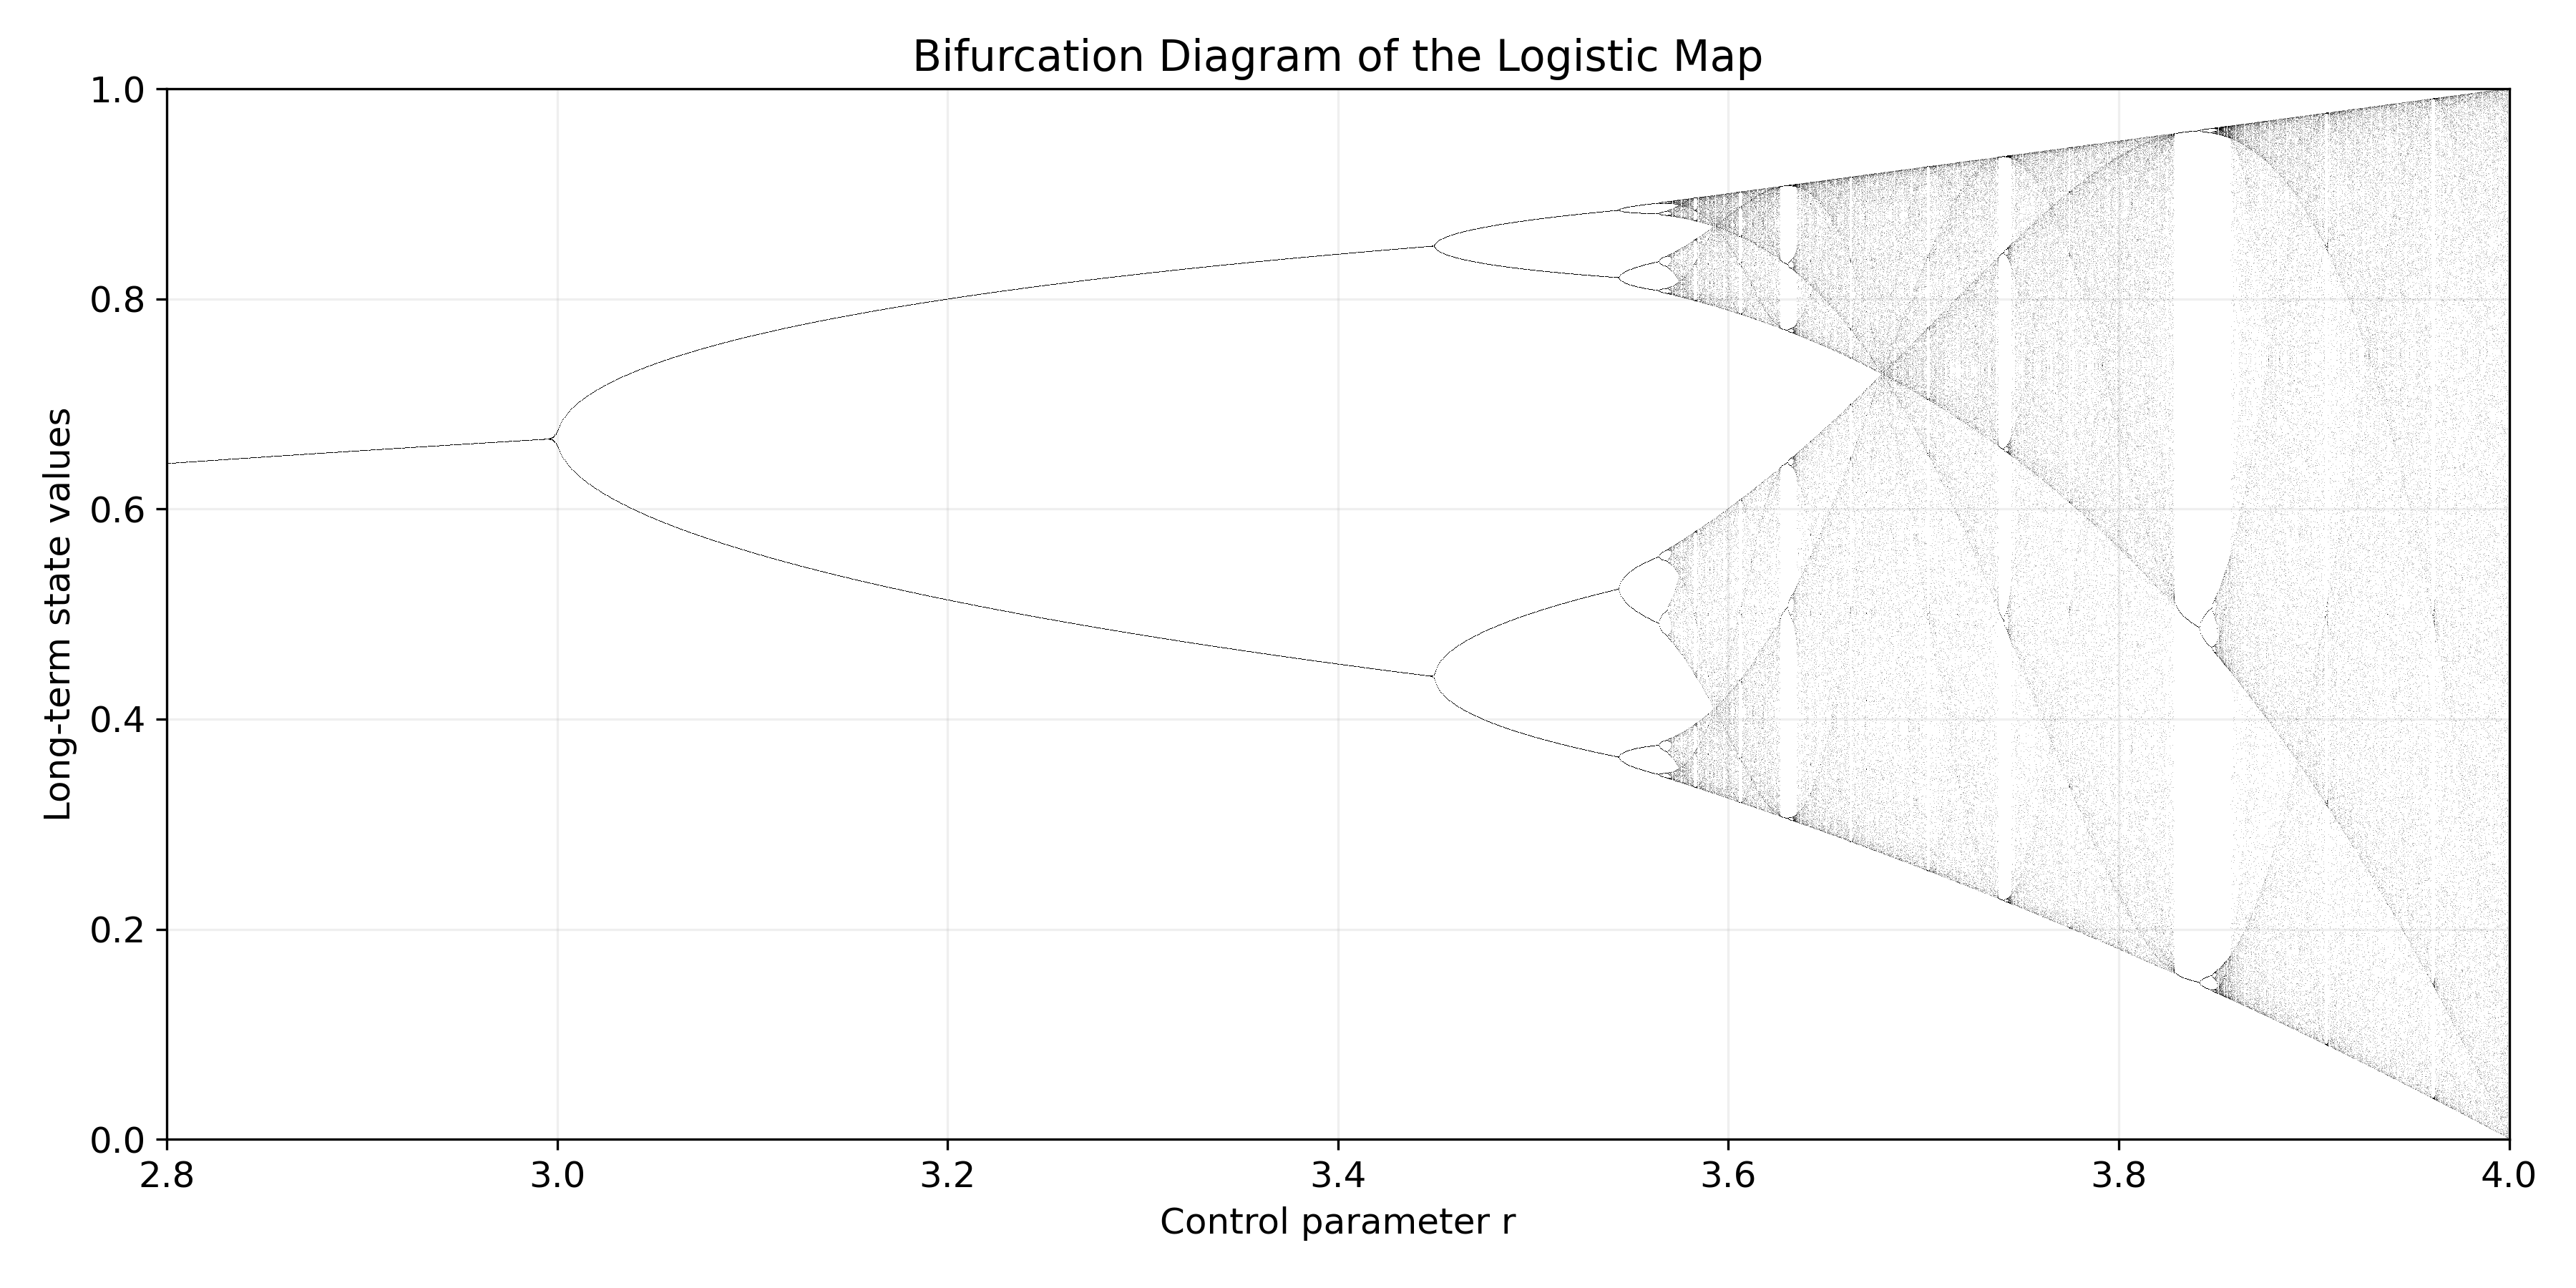
\includegraphics[width=\linewidth]{../results/bifurcation_diagram.png}\\
\captionof{figure}{Bifurcation diagram, $r\in[2.8,4.0]$.}
\end{minipage}\hfill
\begin{minipage}{.49\linewidth}\centering
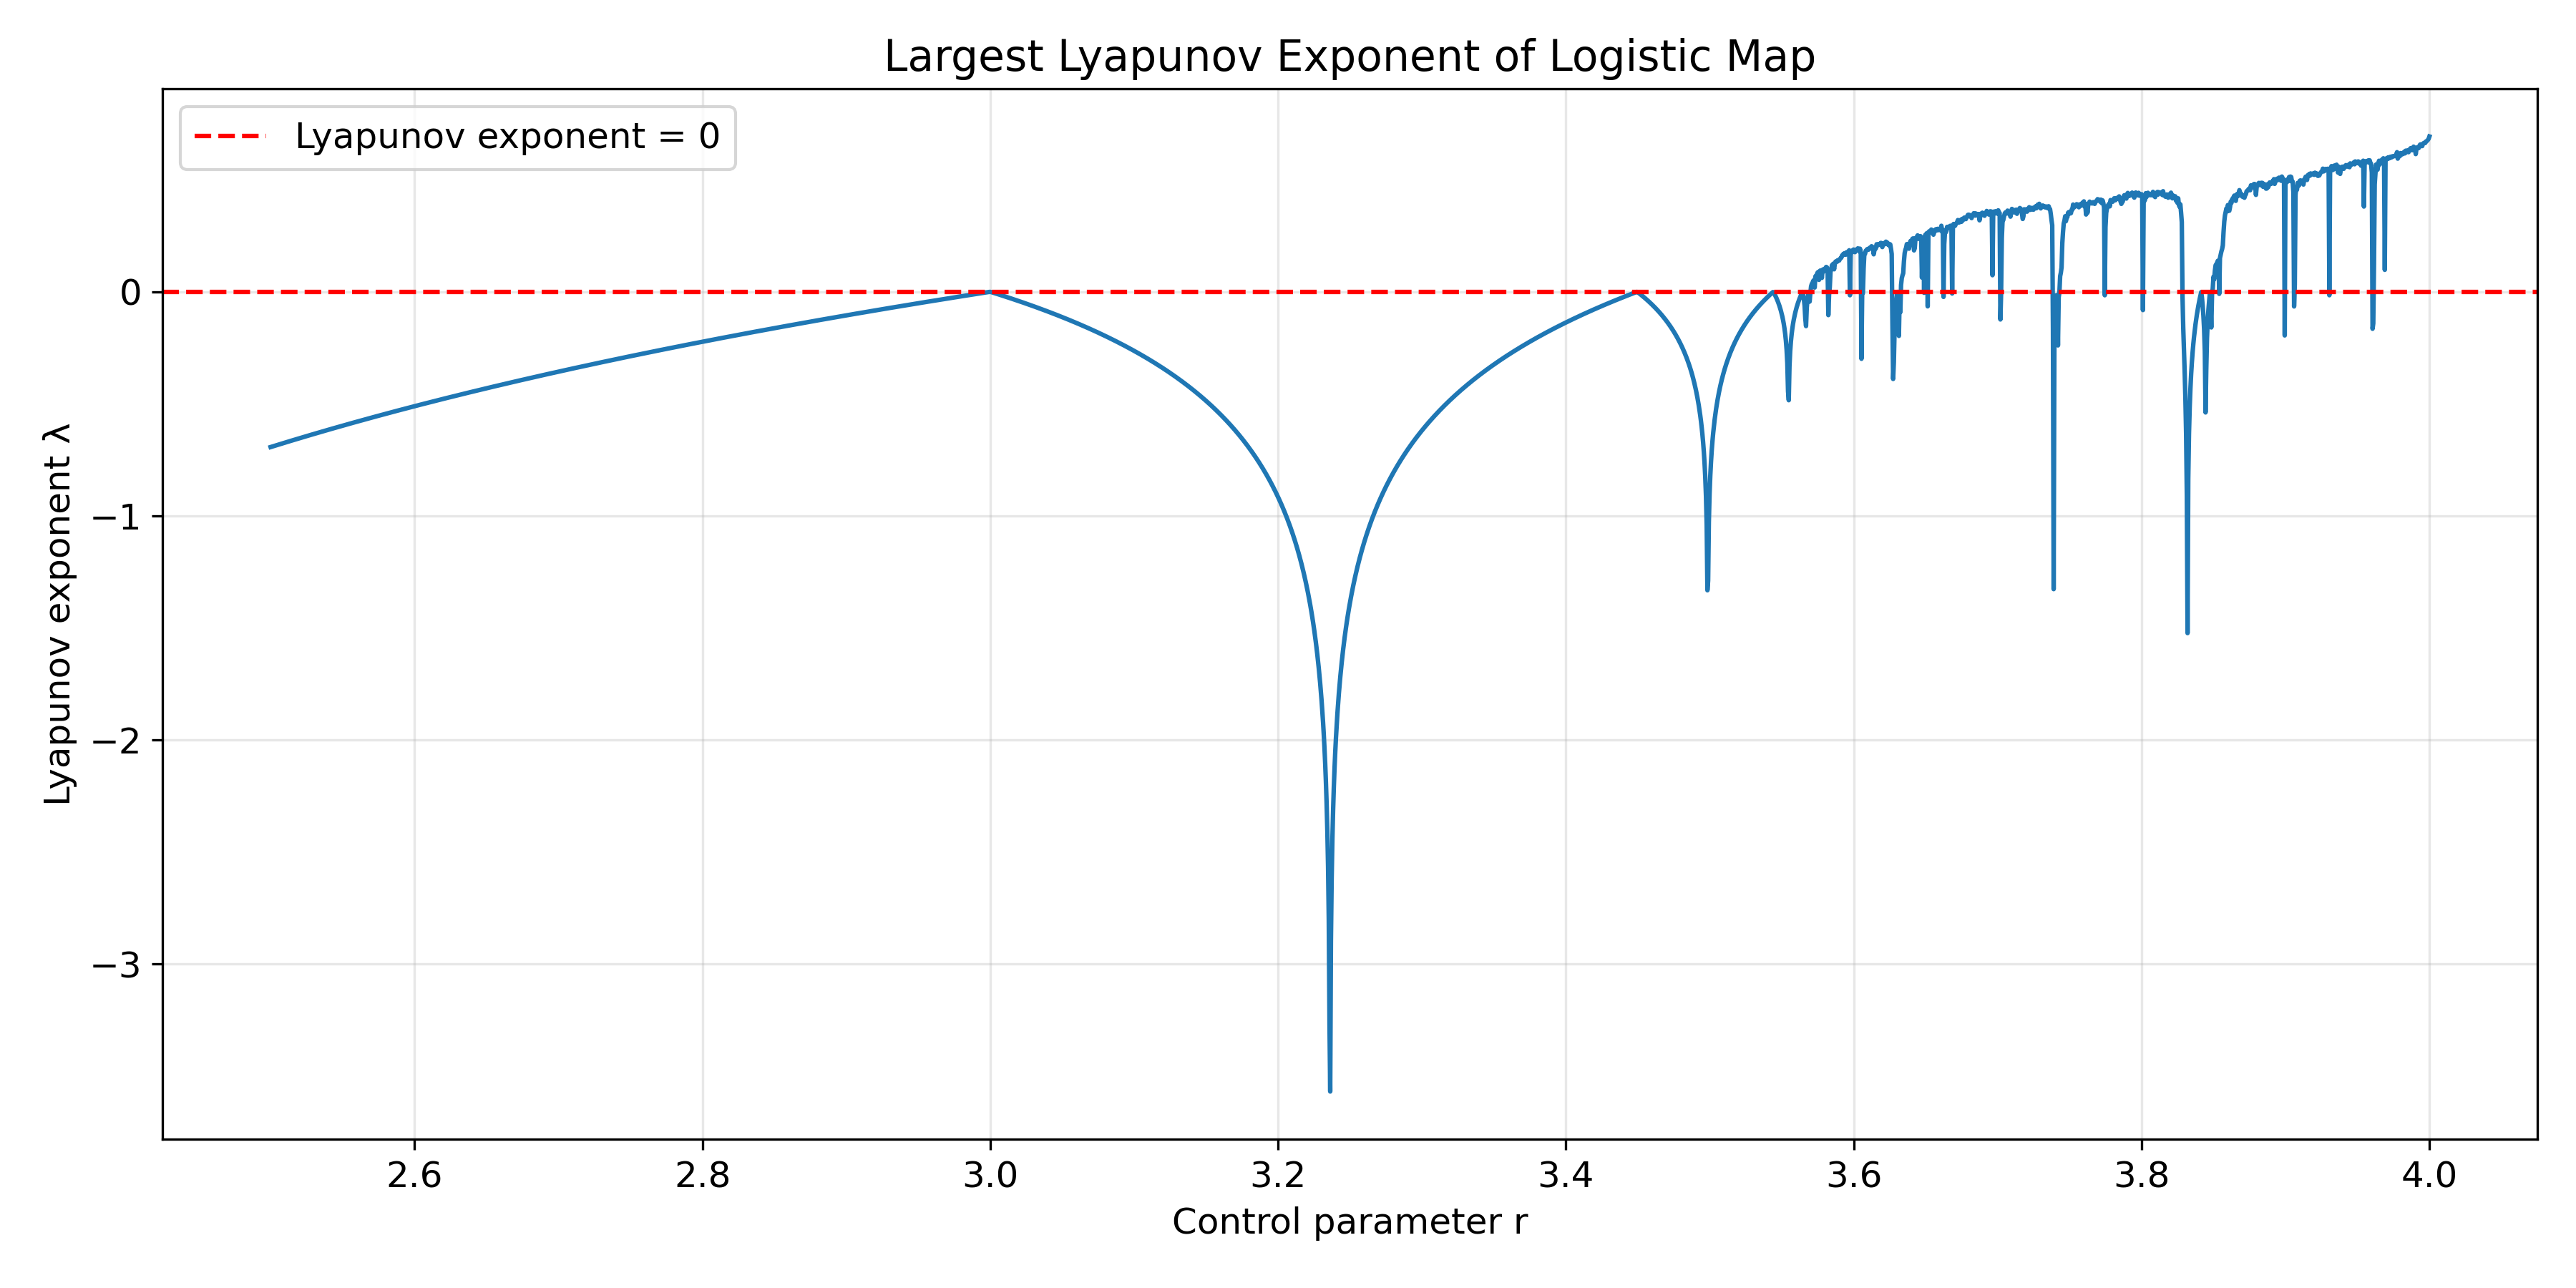
\includegraphics[width=\linewidth]{../results/lyapunov_exponent.png}\\
\captionof{figure}{Numerical largest Lyapunov exponent.}
\end{minipage}
\end{figure}
\clearpage
\begin{figure}[h]
\centering
\begin{minipage}{.49\linewidth}\centering
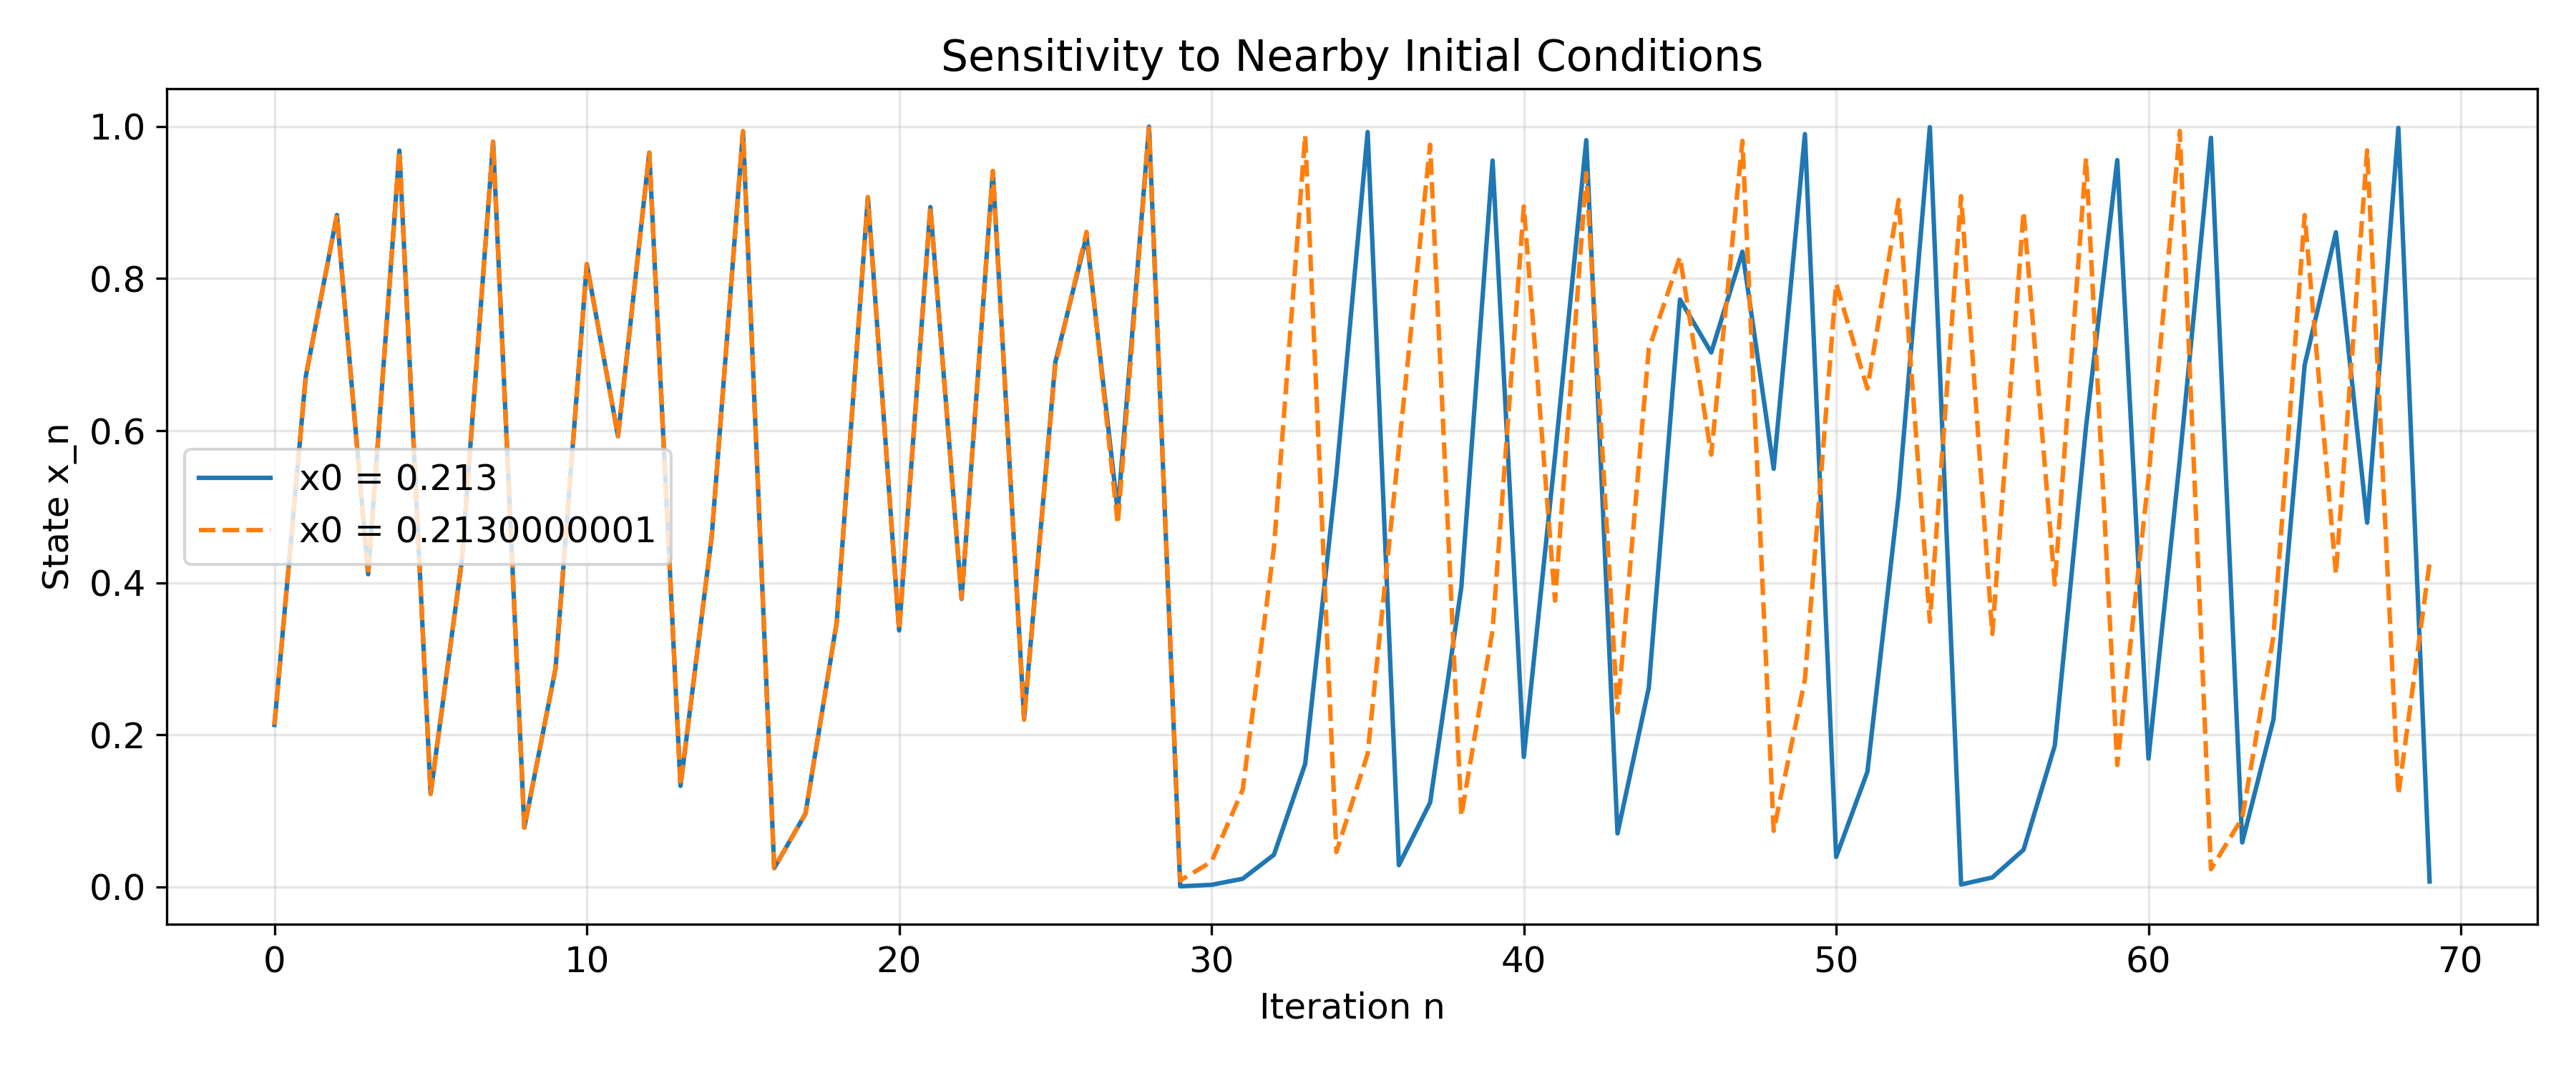
\includegraphics[width=\linewidth]{../results/sensitivity.png}\\
\captionof{figure}{Sensitivity to a $10^{-10}$ perturbation.}
\end{minipage}\hfill
\begin{minipage}{.49\linewidth}\centering
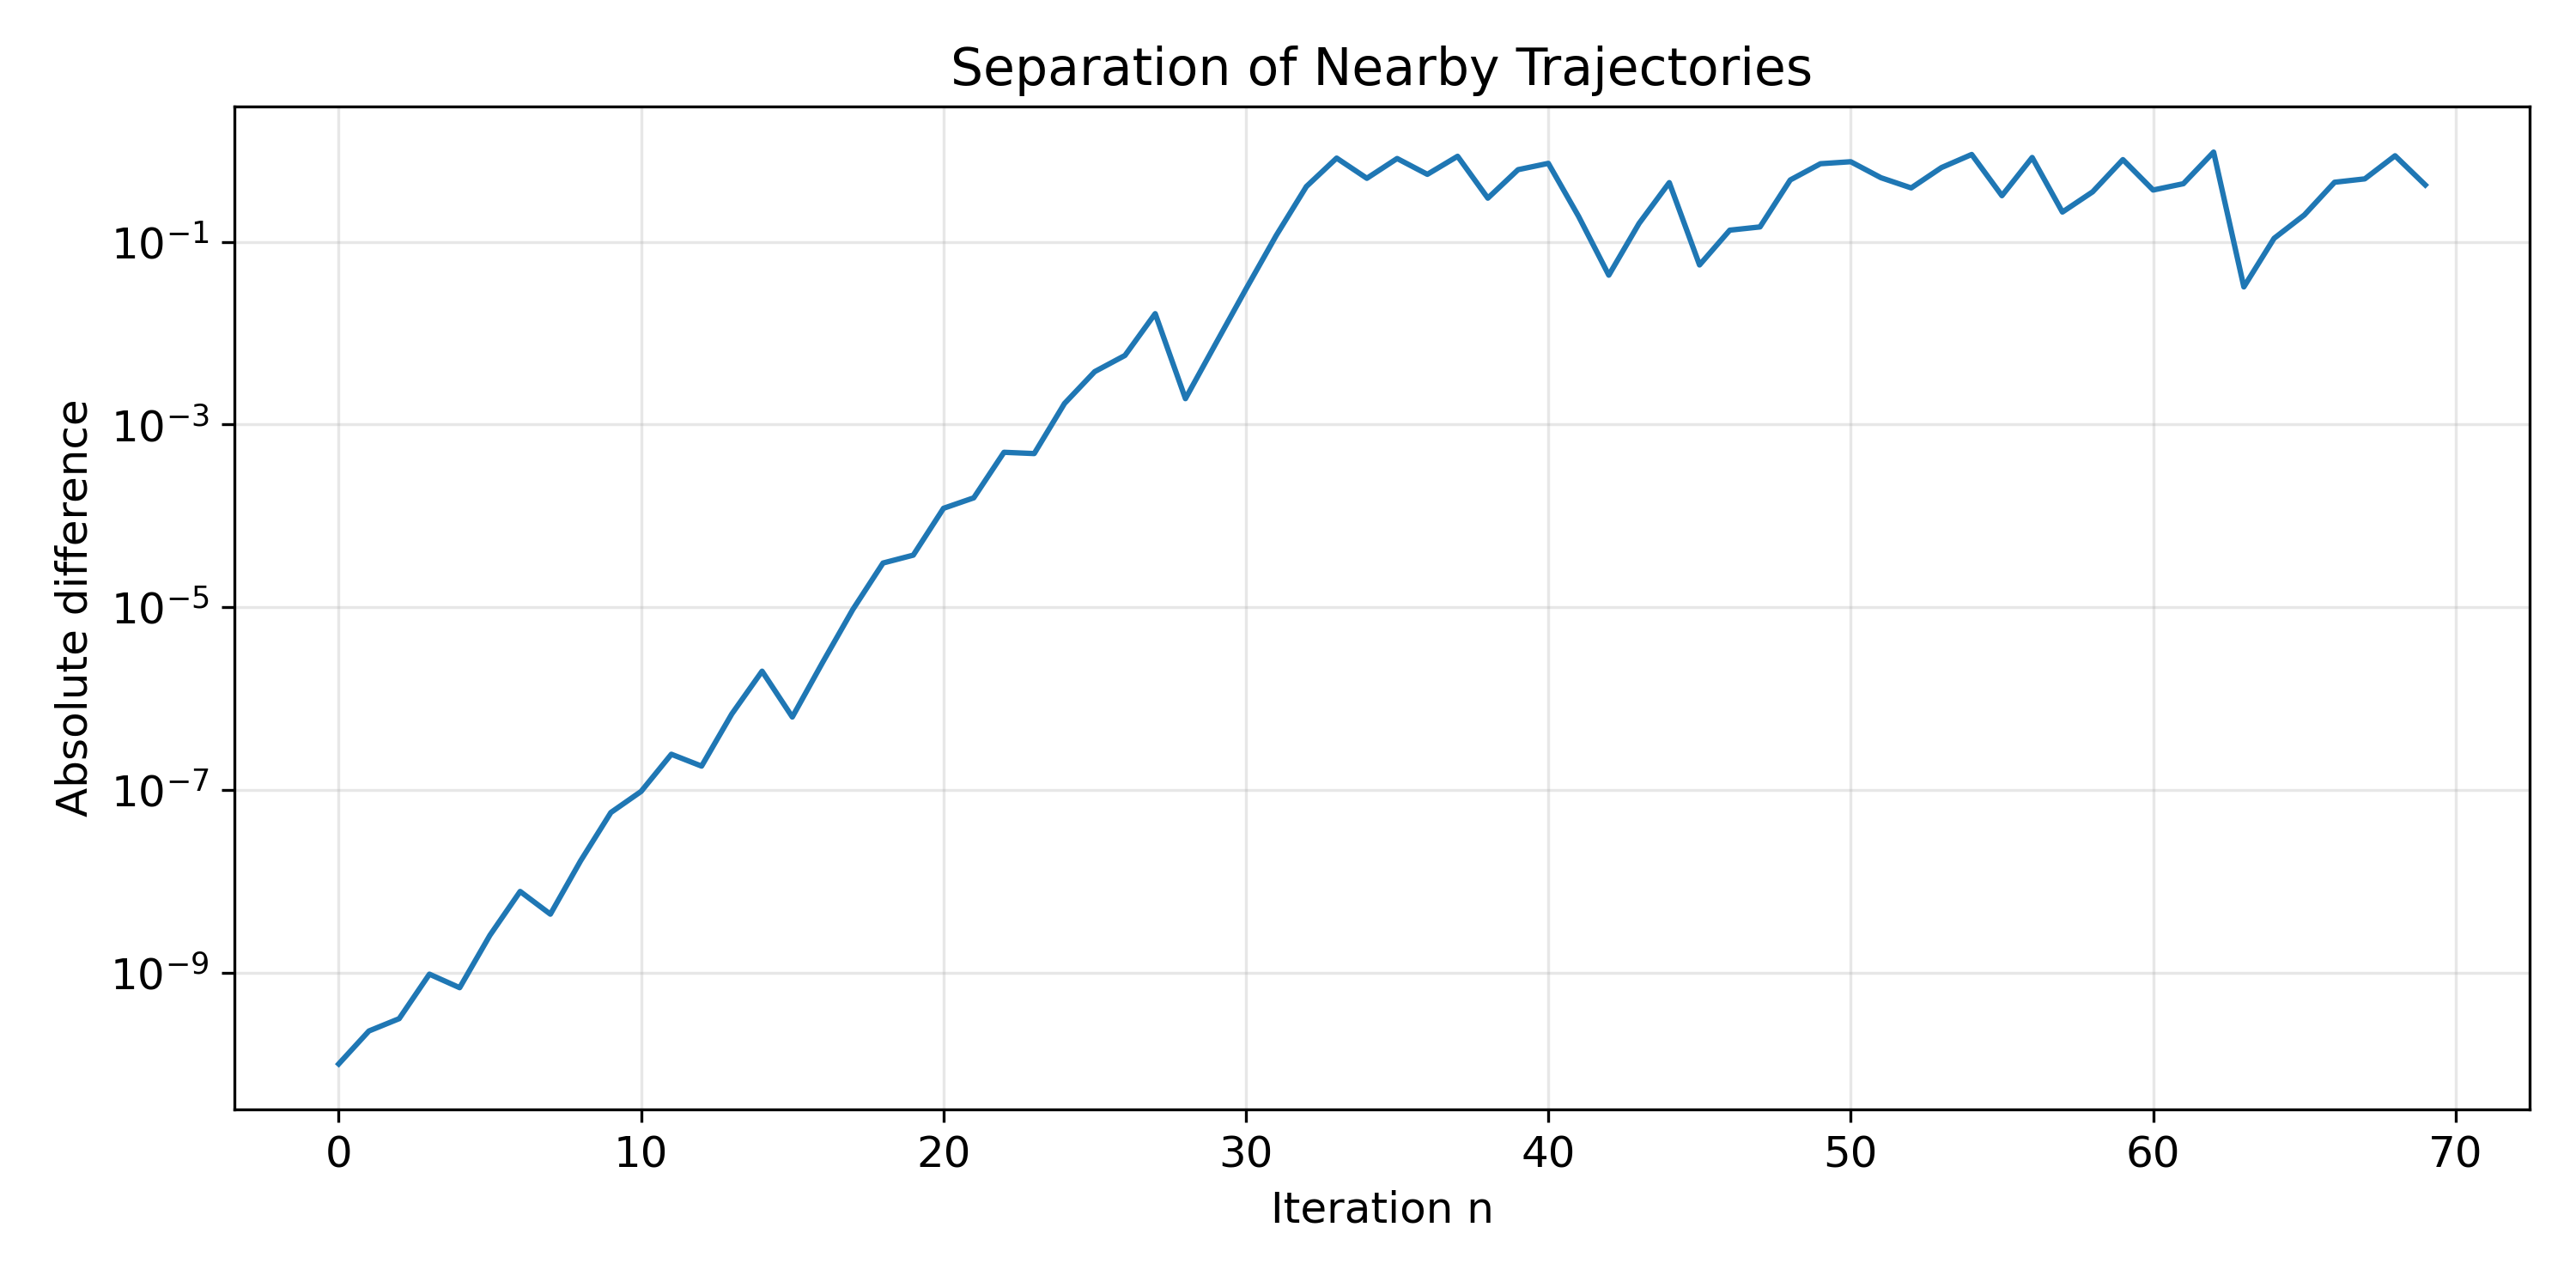
\includegraphics[width=\linewidth]{../results/trajectory_separation.png}\\
\captionof{figure}{Absolute trajectory separation, logarithmic scale.}
\end{minipage}
\end{figure}
\clearpage
\section{Invariant density}
The empirical histogram has the expected U-shaped form and is compared with the analytical invariant density in Figure~\ref{fig:density}. The retained sample mean is 0.4992599, close to the theoretical mean 0.5. This agreement is a numerical consistency check; it does not establish any cryptographic property.
\begin{figure}[h]
\centering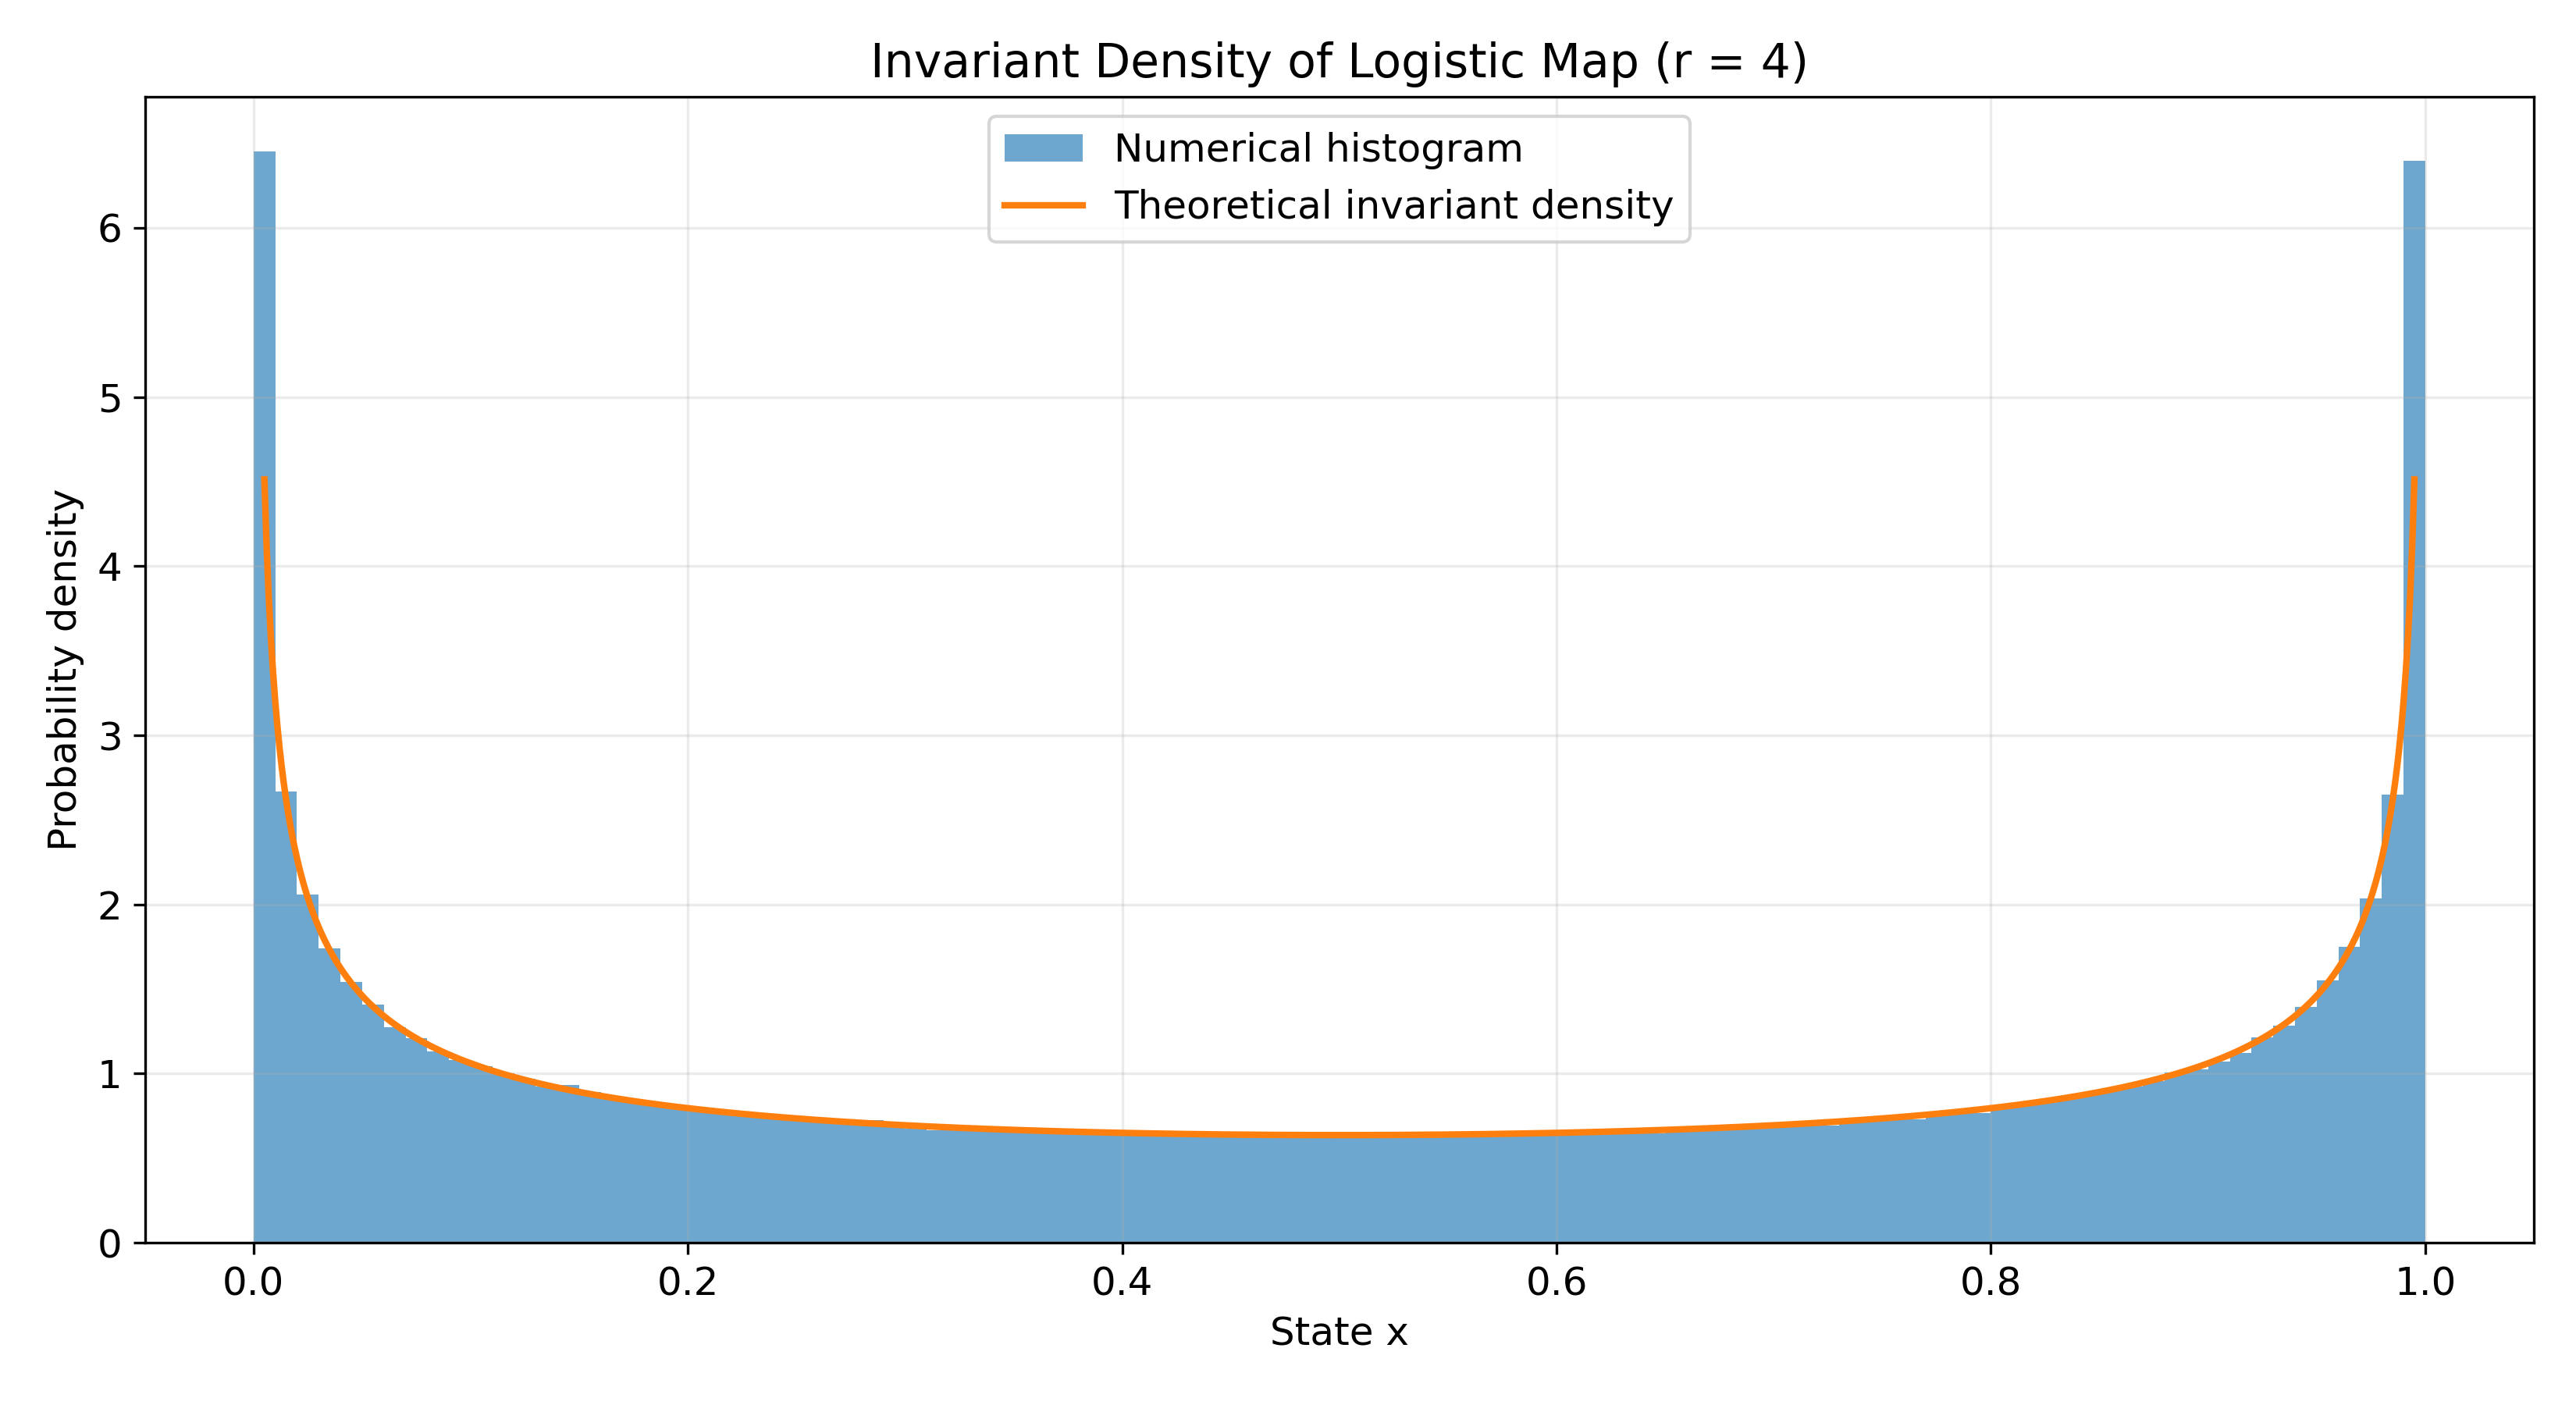
\includegraphics[width=.78\linewidth]{../results/invariant_density.png}
\caption{Numerical histogram and theoretical invariant density at $r=4$.}\label{fig:density}
\end{figure}
\section{Educational interval-mapping text experiment}
The submitted code partitions $[0,1]$ into 26 equal-width intervals for the letters A--Z. For each letter it records how many iterations are needed to reach its interval, then decrypts by replaying the counts from the same initial state. With $r=4.0$ and $x_0=0.213$, the messages \texttt{CHAOS}, \texttt{LOGISTICMAP}, \texttt{NONLINEARDYNAMICS}, and \texttt{ENCRYPTION} were all recovered exactly. Figure~\ref{fig:counts} displays the 43 recorded iteration counts from these checks.
\begin{center}\small
\begin{tabular}{lrrr}\hline
Message & Characters & Recovered & Time (s)\\\hline
CHAOS & 5 & Yes & 0.000212\\
LOGISTICMAP & 11 & Yes & 0.000348\\
NONLINEARDYNAMICS & 17 & Yes & 0.000620\\
ENCRYPTION & 10 & Yes & 0.000360\\\hline
\end{tabular}
\end{center}
\begin{figure}[h]
\centering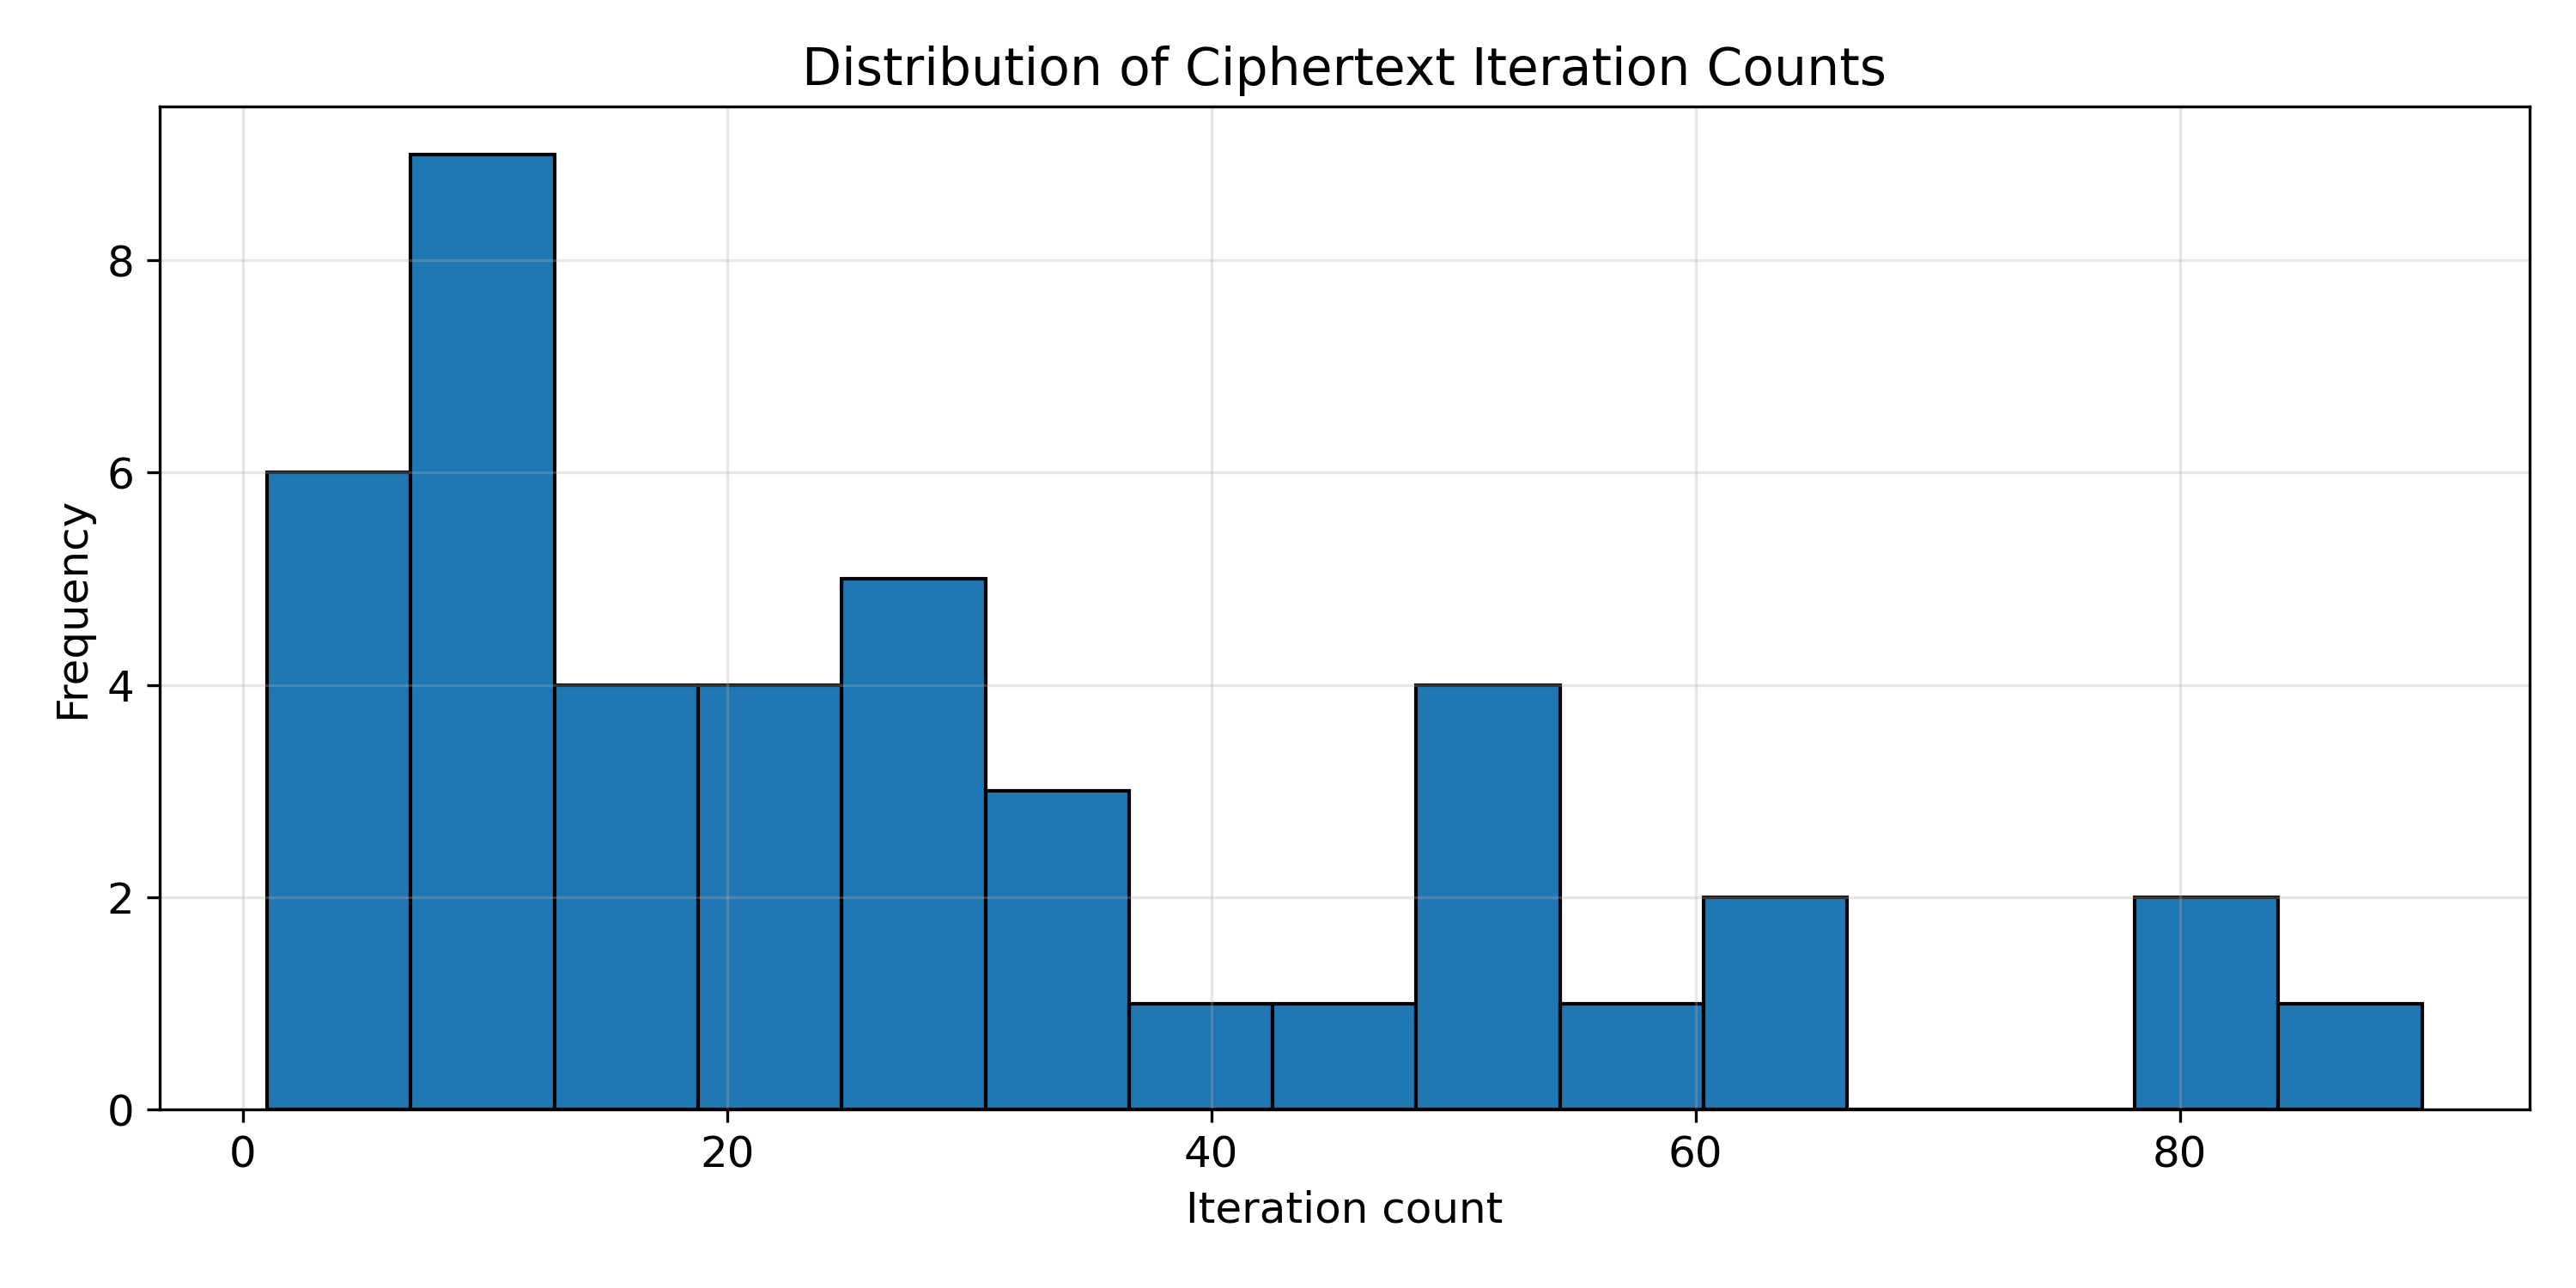
\includegraphics[width=.76\linewidth]{../results/ciphertext_distribution.png}
\caption{Iteration-count distribution for four successful demonstration tests.}\label{fig:counts}
\end{figure}
\section{Literature context, limitations, and conclusion}
\citet{Baptista1998} proposed an iteration-count scheme based on the logistic map's ergodic behaviour. The submitted implementation is not a faithful reproduction: it fixes $r=4$, uses 26 equal-width intervals over the full unit interval, and provides no implementation of the original protocol's full design or keying details. It is therefore not suitable for secure use.

The security statements in this report are literature context, not new experiments. \citet{Alvarez2003} analyse attacks on an ergodic chaotic cipher, and \citet{Li2004} discuss problems and countermeasures for Baptista-type systems. We did \emph{not} reproduce their cryptanalysis, countermeasures, or finite-precision error experiments: the supplied Python script and figures contain logistic-map simulations and four reversible text tests only. The small ciphertext histogram likewise is descriptive, not a statistical security test.

In conclusion, the results demonstrate characteristic nonlinear dynamics and correct recovery for this toy interval mapping. They do not establish confidentiality, resistance to known- or chosen-plaintext attack, or equivalence to the systems in the cited papers. Modern authenticated, standardized cryptography should be used for real data.
\clearpage
% Bibliography is deliberately separate from the five-page main body.
\bibliographystyle{plainnat}
\bibliography{references}
\end{document}
